\documentclass[english, 11 pt, class=article, crop=false]{standalone}
\usepackage[T1]{fontenc}
%\renewcommand*\familydefault{\sfdefault} % For dyslexia-friendly text
\usepackage{lmodern} % load a font with all the characters
\usepackage{geometry}
\geometry{verbose,paperwidth=16.1 cm, paperheight=24 cm, inner=2.3cm, outer=1.8 cm, bmargin=2cm, tmargin=1.8cm}
\setlength{\parindent}{0bp}
\usepackage{import}
\usepackage[subpreambles=false]{standalone}
\usepackage{amsmath}
\usepackage{amssymb}
\usepackage{esint}
\usepackage{babel}
\usepackage{tabu}
\makeatother
\makeatletter

\usepackage{titlesec}
\usepackage{ragged2e}
\RaggedRight
\raggedbottom
\frenchspacing

% Norwegian names of figures, chapters, parts and content
\addto\captionsenglish{\renewcommand{\figurename}{Figur}}
\makeatletter
\addto\captionsenglish{\renewcommand{\chaptername}{Kapittel}}
\addto\captionsenglish{\renewcommand{\partname}{Del}}


\usepackage{graphicx}
\usepackage{float}
\usepackage{subfig}
\usepackage{placeins}
\usepackage{cancel}
\usepackage{framed}
\usepackage{wrapfig}
\usepackage[subfigure]{tocloft}
\usepackage[font=footnotesize,labelfont=sl]{caption} % Figure caption
\usepackage{bm}
\usepackage[dvipsnames, table]{xcolor}
\definecolor{shadecolor}{rgb}{0.105469, 0.613281, 1}
\colorlet{shadecolor}{Emerald!15} 
\usepackage{icomma}
\makeatother
\usepackage[many]{tcolorbox}
\usepackage{multicol}
\usepackage{stackengine}

\usepackage{esvect} %For vectors with capital letters

% For tabular
\usepackage{array}
\usepackage{multirow}
\usepackage{longtable} %breakable table

% Ligningsreferanser
\usepackage{mathtools}
\mathtoolsset{showonlyrefs}

% index
\usepackage{imakeidx}
\makeindex[title=Indeks]

%Footnote:
\usepackage[bottom, hang, flushmargin]{footmisc}
\usepackage{perpage} 
\MakePerPage{footnote}
\addtolength{\footnotesep}{2mm}
\renewcommand{\thefootnote}{\arabic{footnote}}
\renewcommand\footnoterule{\rule{\linewidth}{0.4pt}}
\renewcommand{\thempfootnote}{\arabic{mpfootnote}}

%colors
\definecolor{c1}{cmyk}{0,0.5,1,0}
\definecolor{c2}{cmyk}{1,0.25,1,0}
\definecolor{n3}{cmyk}{1,0.,1,0}
\definecolor{neg}{cmyk}{1,0.,0.,0}

% Lister med bokstavar
\usepackage[inline]{enumitem}

\newcounter{rg}
\numberwithin{rg}{chapter}
\newcommand{\reg}[2][]{\begin{tcolorbox}[boxrule=0.3 mm,arc=0mm,colback=blue!3] {\refstepcounter{rg}\phantomsection \large \textbf{\therg \;#1} \vspace{5 pt}}\newline #2  \end{tcolorbox}\vspace{-5pt}}

\newcommand\alg[1]{\begin{align} #1 \end{align}}

\newcommand\eks[2][]{\begin{tcolorbox}[boxrule=0.3 mm,arc=0mm,enhanced jigsaw,breakable,colback=green!3] {\large \textbf{Eksempel #1} \vspace{5 pt}\\} #2 \end{tcolorbox}\vspace{-5pt} }

\newcommand{\st}[1]{\begin{tcolorbox}[boxrule=0.0 mm,arc=0mm,enhanced jigsaw,breakable,colback=yellow!12]{ #1} \end{tcolorbox}}

\newcommand{\spr}[1]{\begin{tcolorbox}[boxrule=0.3 mm,arc=0mm,enhanced jigsaw,breakable,colback=yellow!7] {\large \textbf{Språkboksen} \vspace{5 pt}\\} #1 \end{tcolorbox}\vspace{-5pt} }

\newcommand{\sym}[1]{\colorbox{blue!15}{#1}}

\newcommand{\info}[2]{\begin{tcolorbox}[boxrule=0.3 mm,arc=0mm,enhanced jigsaw,breakable,colback=cyan!6] {\large \textbf{#1} \vspace{5 pt}\\} #2 \end{tcolorbox}\vspace{-5pt} }

\newcommand\algv[1]{\vspace{-11 pt}\begin{align*} #1 \end{align*}}

\newcommand{\regv}{\vspace{5pt}}
\newcommand{\mer}{\textsl{Merk}: }
\newcommand{\mers}[1]{{\footnotesize \mer #1}}
\newcommand\vsk{\vspace{11pt}}
\newcommand\vs{\vspace{-11pt}}
\newcommand\vsb{\vspace{-16pt}}
\newcommand\sv{\vsk \textbf{Svar} \vspace{4 pt}\\}
\newcommand\br{\\[5 pt]}
\newcommand{\figp}[1]{../fig/#1}
\newcommand\algvv[1]{\vs\vs\begin{align*} #1 \end{align*}}
\newcommand{\y}[1]{$ {#1} $}
\newcommand{\os}{\\[5 pt]}
\newcommand{\prbxl}[2]{
\parbox[l][][l]{#1\linewidth}{#2
	}}
\newcommand{\prbxr}[2]{\parbox[r][][l]{#1\linewidth}{
		\setlength{\abovedisplayskip}{5pt}
		\setlength{\belowdisplayskip}{5pt}	
		\setlength{\abovedisplayshortskip}{0pt}
		\setlength{\belowdisplayshortskip}{0pt} 
		\begin{shaded}
			\footnotesize	#2 \end{shaded}}}

\renewcommand{\cfttoctitlefont}{\Large\bfseries}
\setlength{\cftaftertoctitleskip}{0 pt}
\setlength{\cftbeforetoctitleskip}{0 pt}

\newcommand{\bs}{\\[3pt]}
\newcommand{\vn}{\\[6pt]}
\newcommand{\fig}[1]{\begin{figure}
		\centering
		\includegraphics[]{\figp{#1}}
\end{figure}}

\newcommand{\figc}[2]{\begin{figure}
		\centering
		\includegraphics[]{\figp{#1}}
		\caption{#2}
\end{figure}}

\newcommand{\sectionbreak}{\clearpage} % New page on each section

\newcommand{\nn}[1]{
\begin{equation}
	#1
\end{equation}
}

% Equation comments
\newcommand{\cm}[1]{\llap{\color{blue} #1}}

\newcommand\fork[2]{\begin{tcolorbox}[boxrule=0.3 mm,arc=0mm,enhanced jigsaw,breakable,colback=yellow!7] {\large \textbf{#1 (forklaring)} \vspace{5 pt}\\} #2 \end{tcolorbox}\vspace{-5pt} }
 
%colors
\newcommand{\colr}[1]{{\color{red} #1}}
\newcommand{\colb}[1]{{\color{blue} #1}}
\newcommand{\colo}[1]{{\color{orange} #1}}
\newcommand{\colc}[1]{{\color{cyan} #1}}
\definecolor{projectgreen}{cmyk}{100,0,100,0}
\newcommand{\colg}[1]{{\color{projectgreen} #1}}

% Methods
\newcommand{\metode}[2]{
	\textsl{#1} \\[-8pt]
	\rule{#2}{0.75pt}
}

%Opg
\newcommand{\abc}[1]{
	\begin{enumerate}[label=\alph*),leftmargin=18pt]
		#1
	\end{enumerate}
}
\newcommand{\abcs}[2]{
	\begin{enumerate}[label=\alph*),start=#1,leftmargin=18pt]
		#2
	\end{enumerate}
}
\newcommand{\abcn}[1]{
	\begin{enumerate}[label=\arabic*),leftmargin=18pt]
		#1
	\end{enumerate}
}
\newcommand{\abch}[1]{
	\hspace{-2pt}	\begin{enumerate*}[label=\alph*), itemjoin=\hspace{1cm}]
		#1
	\end{enumerate*}
}
\newcommand{\abchs}[2]{
	\hspace{-2pt}	\begin{enumerate*}[label=\alph*), itemjoin=\hspace{1cm}, start=#1]
		#2
	\end{enumerate*}
}

% Oppgaver
\newcommand{\opgt}{\phantomsection \addcontentsline{toc}{section}{Oppgaver} \section*{Oppgaver for kapittel \thechapter}\vs \setcounter{section}{1}}
\newcounter{opg}
\numberwithin{opg}{section}
\newcommand{\op}[1]{\vspace{15pt} \refstepcounter{opg}\large \textbf{\color{blue}\theopg} \vspace{2 pt} \label{#1} \\}
\newcommand{\ekspop}[1]{\vsk\textbf{Gruble \thechapter.#1}\vspace{2 pt} \\}
\newcommand{\nes}{\stepcounter{section}
	\setcounter{opg}{0}}
\newcommand{\opr}[1]{\vspace{3pt}\textbf{\ref{#1}}}
\newcommand{\oeks}[1]{\begin{tcolorbox}[boxrule=0.3 mm,arc=0mm,colback=white]
		\textit{Eksempel: } #1	  
\end{tcolorbox}}
\newcommand\opgeks[2][]{\begin{tcolorbox}[boxrule=0.1 mm,arc=0mm,enhanced jigsaw,breakable,colback=white] {\footnotesize \textbf{Eksempel #1} \\} \footnotesize #2 \end{tcolorbox}\vspace{-5pt} }
\newcommand{\rknut}{
Rekn ut.
}

%License
\newcommand{\lic}{\textit{Matematikken sine byggesteinar by Sindre Sogge Heggen is licensed under CC BY-NC-SA 4.0. To view a copy of this license, visit\\ 
		\net{http://creativecommons.org/licenses/by-nc-sa/4.0/}{http://creativecommons.org/licenses/by-nc-sa/4.0/}}}

%referances
\newcommand{\net}[2]{{\color{blue}\href{#1}{#2}}}
\newcommand{\hrs}[2]{\hyperref[#1]{\color{blue}\textsl{#2 \ref*{#1}}}}
\newcommand{\rref}[1]{\hrs{#1}{regel}}
\newcommand{\refkap}[1]{\hrs{#1}{kapittel}}
\newcommand{\refsec}[1]{\hrs{#1}{seksjon}}

\newcommand{\mb}{\net{https://sindrsh.github.io/FirstPrinciplesOfMath/}{MB}}


%line to seperate examples
\newcommand{\linje}{\rule{\linewidth}{1pt} }

\usepackage{datetime2}
%%\usepackage{sansmathfonts} for dyslexia-friendly math
\usepackage[]{hyperref}

%\usepackage[T1]{fontenc}
%\renewcommand*\familydefault{\sfdefault} % For dyslexia-friendly text
\usepackage{lmodern} % load a font with all the characters
\usepackage{geometry}
\geometry{verbose,paperwidth=16.1 cm, paperheight=24 cm, inner=2.3cm, outer=1.8 cm, bmargin=2cm, tmargin=1.8cm}
\setlength{\parindent}{0bp}
\usepackage{import}
\usepackage[subpreambles=false]{standalone}
\usepackage{amsmath}
\usepackage{amssymb}
\usepackage{esint}
\usepackage{babel}
\usepackage{tabu}
\makeatother
\makeatletter

\usepackage{titlesec}
\usepackage{ragged2e}
\RaggedRight
\raggedbottom
\frenchspacing

% Norwegian names of figures, chapters, parts and content
\addto\captionsenglish{\renewcommand{\figurename}{Figur}}
\makeatletter
\addto\captionsenglish{\renewcommand{\chaptername}{Kapittel}}
\addto\captionsenglish{\renewcommand{\partname}{Del}}


\usepackage{graphicx}
\usepackage{float}
\usepackage{subfig}
\usepackage{placeins}
\usepackage{cancel}
\usepackage{framed}
\usepackage{wrapfig}
\usepackage[subfigure]{tocloft}
\usepackage[font=footnotesize,labelfont=sl]{caption} % Figure caption
\usepackage{bm}
\usepackage[dvipsnames, table]{xcolor}
\definecolor{shadecolor}{rgb}{0.105469, 0.613281, 1}
\colorlet{shadecolor}{Emerald!15} 
\usepackage{icomma}
\makeatother
\usepackage[many]{tcolorbox}
\usepackage{multicol}
\usepackage{stackengine}

\usepackage{esvect} %For vectors with capital letters

% For tabular
\usepackage{array}
\usepackage{multirow}
\usepackage{longtable} %breakable table

% Ligningsreferanser
\usepackage{mathtools}
\mathtoolsset{showonlyrefs}

% index
\usepackage{imakeidx}
\makeindex[title=Indeks]

%Footnote:
\usepackage[bottom, hang, flushmargin]{footmisc}
\usepackage{perpage} 
\MakePerPage{footnote}
\addtolength{\footnotesep}{2mm}
\renewcommand{\thefootnote}{\arabic{footnote}}
\renewcommand\footnoterule{\rule{\linewidth}{0.4pt}}
\renewcommand{\thempfootnote}{\arabic{mpfootnote}}

%colors
\definecolor{c1}{cmyk}{0,0.5,1,0}
\definecolor{c2}{cmyk}{1,0.25,1,0}
\definecolor{n3}{cmyk}{1,0.,1,0}
\definecolor{neg}{cmyk}{1,0.,0.,0}

% Lister med bokstavar
\usepackage[inline]{enumitem}

\newcounter{rg}
\numberwithin{rg}{chapter}
\newcommand{\reg}[2][]{\begin{tcolorbox}[boxrule=0.3 mm,arc=0mm,colback=blue!3] {\refstepcounter{rg}\phantomsection \large \textbf{\therg \;#1} \vspace{5 pt}}\newline #2  \end{tcolorbox}\vspace{-5pt}}

\newcommand\alg[1]{\begin{align} #1 \end{align}}

\newcommand\eks[2][]{\begin{tcolorbox}[boxrule=0.3 mm,arc=0mm,enhanced jigsaw,breakable,colback=green!3] {\large \textbf{Eksempel #1} \vspace{5 pt}\\} #2 \end{tcolorbox}\vspace{-5pt} }

\newcommand{\st}[1]{\begin{tcolorbox}[boxrule=0.0 mm,arc=0mm,enhanced jigsaw,breakable,colback=yellow!12]{ #1} \end{tcolorbox}}

\newcommand{\spr}[1]{\begin{tcolorbox}[boxrule=0.3 mm,arc=0mm,enhanced jigsaw,breakable,colback=yellow!7] {\large \textbf{Språkboksen} \vspace{5 pt}\\} #1 \end{tcolorbox}\vspace{-5pt} }

\newcommand{\sym}[1]{\colorbox{blue!15}{#1}}

\newcommand{\info}[2]{\begin{tcolorbox}[boxrule=0.3 mm,arc=0mm,enhanced jigsaw,breakable,colback=cyan!6] {\large \textbf{#1} \vspace{5 pt}\\} #2 \end{tcolorbox}\vspace{-5pt} }

\newcommand\algv[1]{\vspace{-11 pt}\begin{align*} #1 \end{align*}}

\newcommand{\regv}{\vspace{5pt}}
\newcommand{\mer}{\textsl{Merk}: }
\newcommand{\mers}[1]{{\footnotesize \mer #1}}
\newcommand\vsk{\vspace{11pt}}
\newcommand\vs{\vspace{-11pt}}
\newcommand\vsb{\vspace{-16pt}}
\newcommand\sv{\vsk \textbf{Svar} \vspace{4 pt}\\}
\newcommand\br{\\[5 pt]}
\newcommand{\figp}[1]{../fig/#1}
\newcommand\algvv[1]{\vs\vs\begin{align*} #1 \end{align*}}
\newcommand{\y}[1]{$ {#1} $}
\newcommand{\os}{\\[5 pt]}
\newcommand{\prbxl}[2]{
\parbox[l][][l]{#1\linewidth}{#2
	}}
\newcommand{\prbxr}[2]{\parbox[r][][l]{#1\linewidth}{
		\setlength{\abovedisplayskip}{5pt}
		\setlength{\belowdisplayskip}{5pt}	
		\setlength{\abovedisplayshortskip}{0pt}
		\setlength{\belowdisplayshortskip}{0pt} 
		\begin{shaded}
			\footnotesize	#2 \end{shaded}}}

\renewcommand{\cfttoctitlefont}{\Large\bfseries}
\setlength{\cftaftertoctitleskip}{0 pt}
\setlength{\cftbeforetoctitleskip}{0 pt}

\newcommand{\bs}{\\[3pt]}
\newcommand{\vn}{\\[6pt]}
\newcommand{\fig}[1]{\begin{figure}
		\centering
		\includegraphics[]{\figp{#1}}
\end{figure}}

\newcommand{\figc}[2]{\begin{figure}
		\centering
		\includegraphics[]{\figp{#1}}
		\caption{#2}
\end{figure}}

\newcommand{\sectionbreak}{\clearpage} % New page on each section

\newcommand{\nn}[1]{
\begin{equation}
	#1
\end{equation}
}

% Equation comments
\newcommand{\cm}[1]{\llap{\color{blue} #1}}

\newcommand\fork[2]{\begin{tcolorbox}[boxrule=0.3 mm,arc=0mm,enhanced jigsaw,breakable,colback=yellow!7] {\large \textbf{#1 (forklaring)} \vspace{5 pt}\\} #2 \end{tcolorbox}\vspace{-5pt} }
 
%colors
\newcommand{\colr}[1]{{\color{red} #1}}
\newcommand{\colb}[1]{{\color{blue} #1}}
\newcommand{\colo}[1]{{\color{orange} #1}}
\newcommand{\colc}[1]{{\color{cyan} #1}}
\definecolor{projectgreen}{cmyk}{100,0,100,0}
\newcommand{\colg}[1]{{\color{projectgreen} #1}}

% Methods
\newcommand{\metode}[2]{
	\textsl{#1} \\[-8pt]
	\rule{#2}{0.75pt}
}

%Opg
\newcommand{\abc}[1]{
	\begin{enumerate}[label=\alph*),leftmargin=18pt]
		#1
	\end{enumerate}
}
\newcommand{\abcs}[2]{
	\begin{enumerate}[label=\alph*),start=#1,leftmargin=18pt]
		#2
	\end{enumerate}
}
\newcommand{\abcn}[1]{
	\begin{enumerate}[label=\arabic*),leftmargin=18pt]
		#1
	\end{enumerate}
}
\newcommand{\abch}[1]{
	\hspace{-2pt}	\begin{enumerate*}[label=\alph*), itemjoin=\hspace{1cm}]
		#1
	\end{enumerate*}
}
\newcommand{\abchs}[2]{
	\hspace{-2pt}	\begin{enumerate*}[label=\alph*), itemjoin=\hspace{1cm}, start=#1]
		#2
	\end{enumerate*}
}

% Oppgaver
\newcommand{\opgt}{\phantomsection \addcontentsline{toc}{section}{Oppgaver} \section*{Oppgaver for kapittel \thechapter}\vs \setcounter{section}{1}}
\newcounter{opg}
\numberwithin{opg}{section}
\newcommand{\op}[1]{\vspace{15pt} \refstepcounter{opg}\large \textbf{\color{blue}\theopg} \vspace{2 pt} \label{#1} \\}
\newcommand{\ekspop}[1]{\vsk\textbf{Gruble \thechapter.#1}\vspace{2 pt} \\}
\newcommand{\nes}{\stepcounter{section}
	\setcounter{opg}{0}}
\newcommand{\opr}[1]{\vspace{3pt}\textbf{\ref{#1}}}
\newcommand{\oeks}[1]{\begin{tcolorbox}[boxrule=0.3 mm,arc=0mm,colback=white]
		\textit{Eksempel: } #1	  
\end{tcolorbox}}
\newcommand\opgeks[2][]{\begin{tcolorbox}[boxrule=0.1 mm,arc=0mm,enhanced jigsaw,breakable,colback=white] {\footnotesize \textbf{Eksempel #1} \\} \footnotesize #2 \end{tcolorbox}\vspace{-5pt} }
\newcommand{\rknut}{
Rekn ut.
}

%License
\newcommand{\lic}{\textit{Matematikken sine byggesteinar by Sindre Sogge Heggen is licensed under CC BY-NC-SA 4.0. To view a copy of this license, visit\\ 
		\net{http://creativecommons.org/licenses/by-nc-sa/4.0/}{http://creativecommons.org/licenses/by-nc-sa/4.0/}}}

%referances
\newcommand{\net}[2]{{\color{blue}\href{#1}{#2}}}
\newcommand{\hrs}[2]{\hyperref[#1]{\color{blue}\textsl{#2 \ref*{#1}}}}
\newcommand{\rref}[1]{\hrs{#1}{regel}}
\newcommand{\refkap}[1]{\hrs{#1}{kapittel}}
\newcommand{\refsec}[1]{\hrs{#1}{seksjon}}

\newcommand{\mb}{\net{https://sindrsh.github.io/FirstPrinciplesOfMath/}{MB}}


%line to seperate examples
\newcommand{\linje}{\rule{\linewidth}{1pt} }

\usepackage{datetime2}
%%\usepackage{sansmathfonts} for dyslexia-friendly math
\usepackage[]{hyperref}

\begin{document}
\section{Grunnprinnsippet}
Selve prinsippet bak sannsynlighetsregning er at vi spør hvor mange \textit{gunstige utfall}  vi har i et utvalg av \textit{mulige utfall}. Sannsynligheten for en \textit{hendelse} er da gitt som et forholdstall mellom disse. \regv
\reg[Sannsynligheten for en hendelse \label{grnprsp}]{
\[ \text{sannsynligheten for en hendelse}=\frac{\text{antall gunstige utfall}}{\text{antall mulige utfall}} \]
} \vsk
Når vi kaster en terning, kaller vi 'å få en firer' en hendelse. Og da en terning har seks forskjellige sider, er det seks mulige utfall.
\fig{san1}
Hvis vi ønsker 'å få en firer', er det bare 1 av disse 6 utfallene som gir oss det vi ønsker, altså er
\[ \text{sannsynlighet for å få en firer}=
 \frac{1}{6} \]
\prbxl{0.6}{For å unngå lange uttrykk bruker vi gjerne enkeltbokstaver for å indikere en hendelse. Istedenfor å skrive 'å få en firer', kan vi bruke bokstaven \textit{F}, og for å indikere at vi snakker om sannsynligheten for en hendelse, bruker vi bokstaven \textit{P}.}\qquad \prbxr{0.3}{$ P $ kommer av det engelske ordet for sannsynlighet, \textit{probability}.} \\[5pt]
Når vi skriver $P(S)$ betyr dette 'sannsynligheten for å få en firer':
\[ P(S)=\frac{1}{6} \]
Hva med det motsatte, altså sannsynligheten for å \textsl{ikke} å få en firer? For å uttrykke at noe er motsatt av en hendelse, setter vi en strek over navnet. Hendelsen 'å \textsl{ikke} få en firer' skriver vi altså som $ \bar{F} $. Det 'å \textsl{ikke} få en firer' er det samme som 'å få \textsl{enten} en ener, en toer, en treer, en femmer \textsl{eller} en sekser', derfor har denne hendelsen 5 gunstige utfall. Det betyr at
\[ P(\bar{S})=\frac{5}{6} \]
\reg[Symboler for sannsynlighet]{
$ P(A) $ er sannsynligheten for at hendelsen $ A $	skjer. \vsk

$ A $ og $ \bar{A} $ er motsatte hendelser. \vsk

$ P(\bar{A}) $ er sannsynligheten for at $ A $ \textsl{ikke} skjer, og omvendt.
} \vsk

\info{Obs!}{
 Som regel er det en god vane å forkorte brøker når det lar seg gjøre, men i sannsynlighetsregning vil det ofte lønne seg å la være. Du vil derfor oppdage at mange brøker i kommende seksjoner kunne vært forkortet.
}
\section{Hendelser med og uten felles utfall}
\subsection{Hendelser uten felles utfall} \vspace{-5pt}
\prbxl{0.6}{La oss kalle hendelsen 'å få en treer' (på en terning) for \textit{T}. Hendelsen 'å få en treer \textsl{eller} en firer' skriver vi da som $ T\cup F $.} \qquad
\prbxr{0.3}{Symbolet \sym{$ \cup $} kalles \textit{union}.}
Det er 2 av 6 sider på en terning som er tre \textsl{eller} fire, sannsynligheten for 'å få en treer \textsl{eller} en firer' er derfor $ \frac{2}{6} $:
\[ P(F\,\cup\,S)=\frac{2}{6} \]
\fig{san1a}

Det samme svaret får vi ved å legge sammen $P(F)$ og $P(S)$:
\[ P(T\,\cup\,F)=P(T)+P(F)=\frac{1}{6}+\frac{1}{6}=\frac{2}{6} \]
Å finne $ P(T\cup F) $ ved å summere $ P(T) $ og $ P(F) $ kan vi gjøre da $ T $ og $ F $ ikke har noen \textit{felles utfall}. Dette fordi ingen sider på trekanten viser \textsl{både} en treer og en firer. \regv

\reg[Hendelser uten felles utfall \label{ufutf}]{For to hendelser \textit{A} og \textit{B} uten felles utfall, er
	\[ P(A\,\cup\,B)=P(A)+P(B) \] \vs\vs}
\newpage
\eks{
Du trekker opp en kule fra en bolle hvor det ligger én rød, to blå og én grønn kule. Hva er sannsynligheten for at du trekker opp en rød \textsl{eller} en blå kule?

\sv
Vi kaller hendelsene 'å få en rød kule' for $ R $ og hendelsen 'å få en blå kule' for $ B $.
\begin{itemize}
	\item Det er i alt 4 mulige utfall (kuler). 
	\item Siden alle kulene bare har én farge, er det ingen av hendelsene $ R $ og $ B $ som har felles utfall.
	\item Sannsynligheten for å trekke en rød kule er
	\[ P(R)=\frac{1}{4} \] 
	\item Sannsynligheten for å trekke en blå kule er
	\[ P(B)=\frac{2}{4} \] 
\end{itemize}
	Sannsynligheten for å få en rød \textsl{eller} en blå kule er dermed 
	 \alg{
		P(R\cup B)&=P(R)+P(B)\br
		&=\frac{1}{4}+\frac{2}{4} \br
		&= \frac{3}{4} 	 
	 }
}
\newpage
\subsection{Summen av alle sannsynligheter er 1}
Tenk at vi kaster en terning og at vi holder både 'å få en firer' og 'å ikke få en firer' for gunstige hendelser . Vi har tidligere sett at $ {P(F)=\frac{1}{6}} $, $ {P(\bar{F})=\frac{5}{6} }$, og at $ F $ og $ \bar{F} $ ikke har felles utfall. Av \rref{ufutf} har vi da at
\algv{
P(F\cup\bar{F})&=P(F)+P(\bar{F})\br
&= \frac{1}{6}+\frac{5}{6} \\
&= 1
}
Enten så skjer $ F $, eller så skjer den ikke. Og skjer den ikke, så skjer $ \bar{F} $. Hvis vi sier at \textsl{både} $ F $ og $ \bar{F} $ er gunstige hendelser, sier vi altså at alle mulige utfall er gunstige, og da gir  \rref{grnprsp} en sannsynlighet lik 1. \regv
 
\reg[Summen av alle sannsynligheter \label{sumer1}]{
Summen av sannsynlighetene for alle mulige hendelser er alltid lik 1.
} \vsk

En hendelse $ A $ og den motsatte hendelsen $ \bar A $ vil til sammen alltid utgjøre alle hendelser. Av \rref{sumer1} har vi da at
\alg{
P(A)+P(\bar{A})&=1 \\
P(A) &= 1-P(\bar{A})
}
\reg[Motsatte hendelser \label{motsatt}]{
For en hendelse $ A $ er
\[ P(A)=1-P(\bar{A}) \]
}
\newpage
\eks{
I en klasse med 25 elever er det 12 jenter og 13 gutter. Èn elev skal tilfeldig trekkes ut til å være med i en matematikkonkurranse. \vsk

\abc{
\item Hva er sannsynligheten for at en gutt blir trukket? 
\item Hva er sannsynligheten for at en gutt \textsl{ikke} blir trukket?}

\sv
Vi kaller hendelsen 'en gutt blir trukket' for $ G $.
\abc{
\item Sannsynligheten for at en gutt blir trukket er
\[ P(G)=\frac{13}{25} \]
\item Sannsynligheten for at en gutt \textsl{ikke} blir trukket er
\alg{P(\bar{G})&=1-P(G) \\
	&=	1-\frac{13}{25} \\
	&= \frac{12}{25}
}
\mer At en gutt \textsl{ikke} blir trukket er det samme som at en jente blir trukket.
}
}
\newpage
\subsection{Felles utfall}	
	Noen ganger er det slik at to hendelser kan ha \textit{felles utfall}. La oss se på en vanlig kortstokk med $52$ kort som er likt delt inn i typene spar, hjerter, ruter og kløver.  Kort som er av sorten knekt, dame, kong eller ess kalles \textit{honnørkort}.	
	\begin{figure}[H]
		\centering
		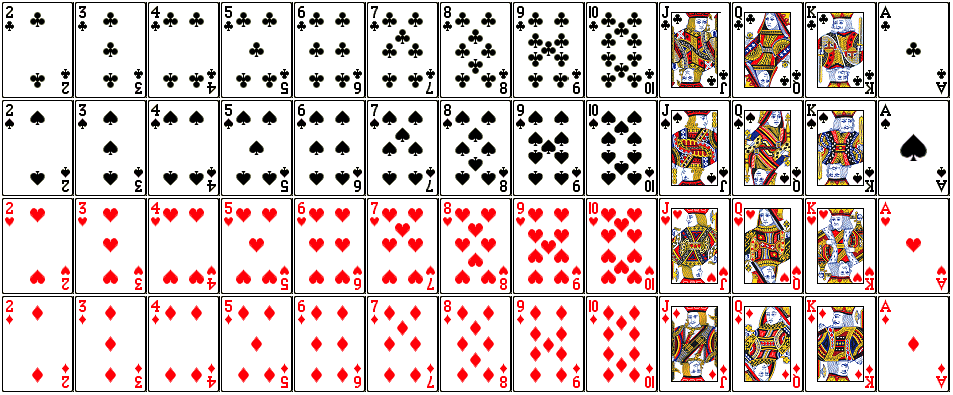
\includegraphics[scale=0.45]{kort}
	\end{figure}  

\prbxl{0.5}{Tenk at vi trekker opp et kort fra en blandet kortstokk. 
	Vi ønsker å finne sannsynligheten for 'å trekke kløverkort \textsl{eller} honnørkort'.
	Vi starter med å telle opp de gunstige utfallene for kløverkort, og finner at antallet er 13.}
\qquad
\prbxr{0.4}{Et kort som kløver kong er et kløverkort, men det er også et honnørkort, og derfor er det begge deler; \textsl{både} kløverkort \textsl{og} honnørkor.}
	
	\begin{figure}[H]
		\centering
		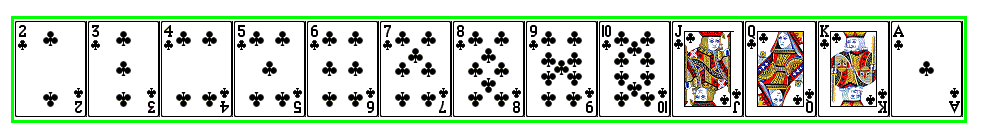
\includegraphics[scale=0.45]{kort1}
	\end{figure}
	Etterpå teller vi opp gunstige utfall for honnørkort, og finner at 
	antallet er 16. \\
	\begin{figure}[H]
		\centering
		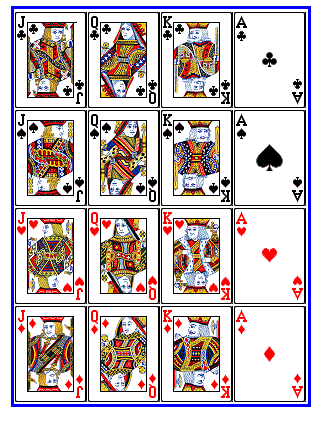
\includegraphics[scale=0.45]{kort2}
	\end{figure}
Til sammen har vi telt ${13+16=29}$ gunstige utfall, men nå støter vi på et problem. For da vi fant alle kløverkort, telte vi blant andre kløver knekt, dame, kong og ess. Disse fire kortene telte vi også da vi fant alle honnørkort, noe som betyr at vi har telt de samme kortene to ganger! \\
	\begin{figure}[H]
		\centering
		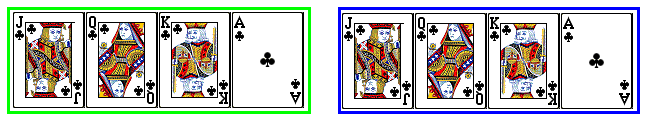
\includegraphics[scale=0.45]{kort4}
	\end{figure}
Det finnes jo for eksempel ikke to kløver ess i en kortstokk, så skal vi regne ut hvor mange kort som oppfyller kravet om å være kløver \textsl{eller} honnør, så må vi trekke ifra antallet kort vi har telt dobbelt:
$$ 13+16-4=25 $$
	\begin{figure}[H]
		\centering
		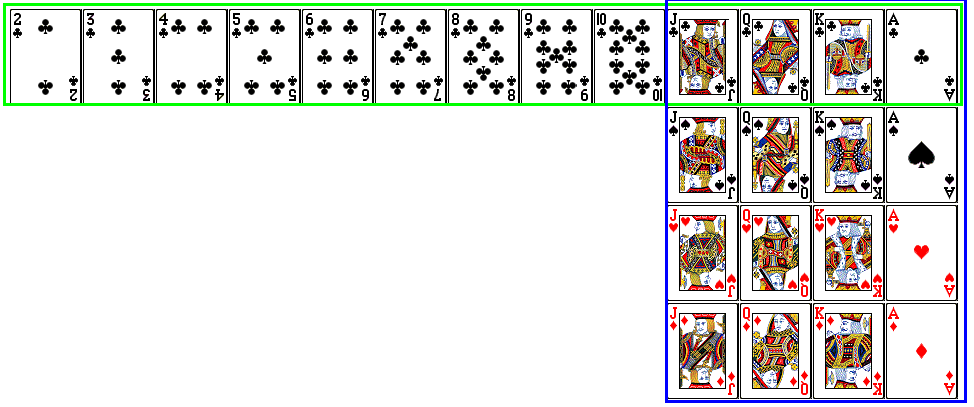
\includegraphics[scale=0.45]{kort3}
	\end{figure}

La \textit{K} være hendelsen 'å trekke et kløverkort' og \textit{H} være hendelsen 'å trekke et honnørkort'. Siden det er 25 kort som er kløverkort \textsl{eller} honnørkort av i alt 52 kort, har vi at
$$P(K\cup\,H)=\frac{25}{52}$$

Siden vi har 13 kløverkort og 16 honnørkort, får vi videre at
$$P(K)=\frac{13}{52} \text{\; og \;} P(H)=\frac{16}{52}$$
\prbxl{0.6}{
Vi har sett at fire kort er \textsl{både} kløver \textsl{og} honnørkort, dette skriver vi som}\qquad
\prbxr{0.3}{Symbolet \sym{$ \cap $} kalles \textit{snitt}.} \vs
\[ K\,\cap\,H=4 \]
Vi sier da at \textit{K} og \textit{H} har 4 \textit{felles utfall}.
Videre er
\[ P(K\,\cap\,H)=\frac{4}{52} \]

Nå som vi har funnet $ P(K), P(H)$ og $P(K\cup H)$ kan vi igjen finne  $P(K\,\cap\,H)$ på følgende måte:
\begin{align*}
P(K\,\cup\,H)&=P(K)+P(H)-P(K\,\cap\,H) \br
&= \frac{13}{52}+\frac{16}{52}-\frac{4}{52} \br
&= \frac{25}{52}
\end{align*}

\reg[Hendelser med felles utfall \label{mfutf}]{For to hendelser $ A $ og $ B $ er
	\[ P(A\,\cup\,B)=P(A)+P(B)-P(A\,\cap\,B) \]\vs\vs}
\info{Merk}{
	Hvis man anvender \rref{mfutf} på to hendelser uten felles utfall, ender man opp med \rref{ufutf}. 
}
\newpage
\eks{ \label{eksfothand}
I en klasse på 20 personer spiller 7 personer fotball og 10 personer spiller handball. Av disse er det 4 som spiller både fotball og handball. Om man trekker ut én person fra klassen, hva er sannsynligheten for at denne personen spiller fotball \textsl{eller} handball?
		
\sv
Vi lar $ F $ være hendelsen 'spiller fotball' og $ H $ være hendelsen 'spiller handball'.
\begin{itemize} 
\item Sannsynligheten for at en person spiller fotball er
\[ P(F)=\frac{7}{20} \]
\item Sannsynligheten for at en person spiller handball er
\[ P(H)=\frac{10}{20} \]
\item Sannsynligheten for at en person spiller \textsl{både} fotball og handball er
\[ P(F\cap H)=\frac{4}{20} \]	
\end{itemize}

Sannsynligheten for at en person spiller fotball \textsl{eller} handball er derfor \alg{
P(F\cup H)&= P(F)+P(H)-P(F\cap H)\br
&=\frac{7}{20}+\frac{10}{20}-\frac{4}{20}\br
&=\frac{13}{20}
} 
}

\subsection{Venndiagram}
Målet med et venndiagram er å lage en figur som illustrerer antallet av de \textsl{særskilte} utfallene og de \textsl{felles} utfallene. La oss bruke eksempelet på side \pageref{eksfothand} til å lage en slik figur. For klassen der noen spiller fotball, noen handball og noen begge deler, kan vi lage et venndiagram som vist under.
\begin{figure}
	\centering
	\includegraphics[]{\figp{venn}}
\end{figure}
Den grønne ellipsen\footnote{En ellipse er en ''strekt'' sirkel.} representerer de som spiller fotball ($ F $) og den blå de som spiller handball ($ H $). Da noen spiller \textsl{begge} sportene ($ F\cap H $), har vi tegnet ellipsene litt over i hverandre. Videre vet vi at 7 spiller fotball, 10 spiller handball og 4 av disse gjør \textsl{begge }deler. Dette illustreres slik:
\begin{figure}
	\centering
	\includegraphics[]{\figp{vennb}}
\end{figure}
Diagrammet forteller nå at 3 personer spiller \textsl{bare} fotball og 6 spiller \textsl{bare} handball. I tilleg spiller 4 personer \textsl{både} fotball og handball. (Til sammen er det derfor 7 som spiller fotball og 10 som spiller handball.) 
\newpage
\eks[1]{I en skoleklasse er det 31 elever. I denne klassen er det 15 elever som tar buss til skolen og 9 elever som tar båt. Av disse er det 3 stykker som tar både buss og båt.

\abc{
\item Sett opp et venndiagram som illustrerer gitt informasjon.\br

\item Én person trekkes tilfeldig ut av klassen. Hva er sannsynligheten for at denne personen tar buss \textsl{eller} båt til skolen?
}
\sv
\abc{
\vs	
\item Siden 3 elever tar \textsl{både} buss og båt, er det \y{15-3=12} som \textsl{bare} tar buss og \y{9-3=6} som \textsl{bare} tar båt. Vi lar $ A $ bety 'tar buss' og $ B $ bety 'tar båt', venndiagrammet vårt blir da seende slik ut:
\fig{venne}
\item Sannsynligheten for at en person tar buss \textsl{eller} båt kan vi skrive som \y{P(A\cup B) }. Siden 15 elever tar buss, 9 tar båt og 3 tar begge deler, er det i alt \y{15+9-3=21} elever som tar buss \textsl{eller} båt. Da det er 31 elever i alt å velge mellom, er
\[ P(A\cup B)=\frac{21}{31} \]\vs}
}
\newpage
\eks[2]{
Om en klasse med 29 elever vet vi følgende:
\begin{itemize}
	\item 16 elever spiller fotball
	\item 12 elever spiller handball
	\item 7 elever spiller volleyball
	\item 5 elever spiller både fotball og handball, men ikke volleyball
	\item 3 elever spiller både fotball og volleyball, men ikke handball
	\item 2 elever spiller både handball og volleyball, men ikke fotball.	
	\item 1 elev spiller alle tre sportene.
\end{itemize}
\textbf{a)} Sett opp et venndiagram som beskriver fordelingen av de tre sportene i klassen.\br

\textbf{b)} Én person trekkes tilfeldig ut av klassen. Hva er sannsynligheten for at denne personen spiller enten fotball, handball eller volleyball?\br

\textbf{c)} Personen som trekkes ut viser seg å spille fotball. Hva er sjansen for at denne personen også spiller handball?

\sv
La $ F $ bety 'spiller fobtall', $ H $ bety 'spiller handball' og $ V $ bety 'spiller volleyball'. Når vi skal lage et venndiagram, er det lurt å skrive inn de felles utfallene først. Ut ifra fjerde til syvende punkt kan vi tegne dette:
\begin{figure}
	\centering
	\includegraphics[]{\figp{venn3ea}}
\end{figure}
Da ser vi videre at \y{16-5-1-3=7} elever spiller \textsl{bare} fotball, \y{12-5-1-2=4} spiller \textsl{bare} handball og \y{9-3-1-2=3} spiller \textsl{bare} volleyball:
\begin{figure}
	\centering
	\includegraphics[]{\figp{venn3e}}
\end{figure} 
\textbf{b)} Av diagrammet vårt ser vi at det er $ 8+5+1+3+4+2+3= 26 $ unike elever som spiller én eller flere av sportene. Sjansen for å trekke en av disse 26 i en klasse med 29 elever er $ \frac{26}{29} $. \br

\textbf{c)} Vi leser av diagrammet at av de totalt 16 som spiller fotball, er det \y{5+1=6} som også spiller handball. Sjansen for at personen som er trukket ut spiller handball er derfor $ \frac{6}{16}=\frac{3}{8} $.
}
\subsection{Krysstabell}
Når det er snakk om to hendelser, kan vi også sette opp en \textit{krysstabell} for å skaffe oss oversikt. Si at det på en skole med 300 elever deles ut melk og epler til de elevene som ønsker det i lunsjen. Si videre at 220 av elevene får melk, mens 250 får eple. Av disse er det 180 som får både melk og eple. Hvis vi lar $ M $ bety \textit{får melk} og $ E $ bety \textit{får eple}, vil krysstabellen vår først se slik ut:
\begin{center}
	\renewcommand{\arraystretch}{1.5}
	\begin{tabular}{|c|c|c|c}
		& M &$ \bar{M} $ & sum \\
		\hline$ E $ & & \\
		\hline$ \bar{E} $ & &\\
		\hline sum & &
	\end{tabular}
\end{center}
Så fyller vi inn tabellen ut ifra infoen vi har:
\begin{itemize}
	\item får \textsl{både} melk og eple: \y{M\cap E = 180}
	\item får melk, men ikke eple: \y{M\cap \bar{E} = 220-180=40}
	\item får eple, men ikke melk: \y{E\cap M=250-180=70}
	\item får hverken melk eller eple: \y{\bar M \cap\bar{E}=300-180-40-70=10}
\end{itemize}

\begin{center}
	\renewcommand{\arraystretch}{1.5}
	\begin{tabular}{|c|c|c|c}
				& M &$ \bar{M} $ & sum \\
		\hline$ E $ & 180& 70&250 \\
		\hline$ \bar{E} $ & 40 &10&50\\
		\hline sum & 220& 80& 300
	\end{tabular}
\end{center}

\section{Gjentatte trekk \label{komb}}
\subsection{Permutasjoner}
\begin{figure}[H]
	\centering
	\includegraphics[scale=0.8]{\figp{bolle}}
	\vs
\end{figure}
Si vi har en bolle med fire kuler som er nummererte fra 1 til 4. I et forsøk trekker vi opp en og en kule fram til vi har trukket opp tre kuler. Hvis vi for eksempel først trekker kule 2, deretter kule 4, og så kule 3, får vi \textit{permutasjonen} $2\; 4\; 3$. \vsk
 
Hvor mange forskjellige permutasjoner kan vi få? La oss lage en figur som hjelper oss med å finne svaret. Ved første trekning er det 4 kuler å plukke av, vi kan derfor si at vi har 4 veier å gå. Enten trekker vi kule 1, eller kule 2, eller kule 3, eller kule 4:
\begin{figure}[H]
\centering
\includegraphics[scale=0.8]{\figp{perm1a}}
\end{figure}
Kula vi trekker opp, legger vi ut av bollen, og trekker så for andre gang. For hver av de 4 veiene vi kunne gå i første trekning får vi nå 3 nye veier å gå. Altså har vi nå  $3\cdot4=12$ veier vi kan gå.

\begin{figure}[H]
	\centering
	\includegraphics[scale=0.8]{\figp{perm1b}}
\end{figure}
 
Den andre kula vi trekker opp legger vi også ut av bollen,  så  for hver av de 12 veiene fra 2. trekning, får vi nå to nye mulige veier å gå. Totalt antall veier (permutasjoner) blir derfor $12\cdot2=24$. 

\begin{figure}[H]
\centering
\includegraphics[scale=0.8]{\figp{perm1c}}
\end{figure}

Denne utregningen kunne vi også ha skrevet slik:
\[ 4\cdot3\cdot2=24 \]
\reg[Produktregelen for permutasjoner]{Når vi foretar flere trekninger etter hverandre, finner vi alle mulige permutasjoner ved å gange sammen antall mulige utfall i hver trekning.
}

\eks{	
	Av de 29 bokstavene i alfabetet ønsker vi å lage et ord som består av 3 bokstaver. Vi godkjenner ord som ikke har noen betydning, men en bokstav kan bare brukes én gang i ordet.\os
	
	Hvor mange ord kan vi lage?

	\sv
	Først har vi 29 bokstaver å trekke fra, deretter 28 bokstaver, og til slutt 27 bokstaver. Dermed er antall permutasjoner gitt som
	\[ \underbrace{29}_{\substack{\text{mulige utfall}\\\text{1. trekning}}}\cdot\underbrace{28}_{\substack{\text{mulige utfall}\\\text{2. trekning}}}\cdot\underbrace{27}_{\substack{\text{mulige utfall}\\\text{3. trekning}}}=21\,924 \]
	Vi kan altså lage 21\,924 forskjellige ord.
}
\eks[2]{
	Vi kaster om krone eller mynt fire ganger etter hverandre. Hvor mange permutasjoner har vi da?
	
	\sv
	Hver gang vi kaster om krone eller mynt, har vi to mulige utfall. Antall permutasjoner er derfor gitt som
	\[ 2\cdot2\cdot2\cdot2=16 \]\vs}
\newpage
\info{Kombinasjoner}{
I dagligtale blir ofte ordet \textit{kombinasjoner} brukt istedenfor permutasjoner, men innenfor sannsynlighetsregning har kombinasjoner og permutasjoner forskjellig betydning. Den store forskjellen er at permutasjoner tar hensyn til rekkefølge, mens kombinasjoner ikke gjør det. \vsk

Si vi ønsker å danne et ord med to bokstaver ved hjelp av med bokstavene $ A $, $ B $ og $ C $, og at vi godtar gjenbruk av bokstav. Da har vi 9 mulige permutasjoner:
\[ AA, AB, AC, BB, BA, BC, CC, CA, CB \]
Kombinasjoner derimot viser til en unik sammensetting når rekkefølge ikke tas hensyn til, for eksempel er $ AB $ og $ BA $ den samme kombinasjonen. I dette tilfellet har vi altså 6 kombinasjoner
\[ AA, AB, AC, BB, BC, CC \]
}
\newpage
\subsection{Sannsynlighet ved gjentatte trekk}
\prbxl{0.5}{Tenk at vi har en med bolle sju kuler. Tre av dem er grønne, to er blå og to er røde. Si at vi tar opp først én kule av bollen, og deretter én til. Hva er sannsynligheten for at vi trekker opp to grønne kuler?} \qquad
\fgbxr{0.4}{
\fig{bolle2}
}
Hvis vi lar $ G $ bety 'å trekke en grønn kule', kan vi skrive denne sannsynligheten som $ P(GG) $. For å komme fram til et svar, starter vi med å finne ut hvor mange \textsl{gunstige} permutasjoner vi har. Siden vi i første trekning har 3 gunstige utfall, og i andre trekning 2 gunstige utfall, har vi $3\cdot2=6$ gunstige permutasjoner. Totalt velger vi blant 7 kuler i første trekning og 6 kuler i andre trekning. Antall \textsl{mulige} permutasjoner er derfor $7\cdot6=42$\,. Sannsynligheten for å få to grønne kuler blir da
\begin{equation}
P(GG)=\frac{3\cdot2}{7\cdot6}=\frac{6}{42}=\frac{1}{7} \label{trekk}
\end{equation}
\rule{\linewidth}{1pt}
La oss også finne sannsynligheten for å få en grønn kule for hver trekning isolert sett. I første trekning har vi 3 grønne av i alt 7 kuler, altså er
\[ P(G)=\frac{3}{7} \]
\prbxl{0.5}{I andre trekning tas det for gitt at en grønn kule er plukket opp ved første trekning, og dermed er ute av bollen. Vi har da 2 av 6 kuler som er grønne:
\[ P(G|G)=\frac{2}{6} \]
}
\qquad
\prbxr{0.4}{Symbolet \sym{$ | $} betyr \textit{\textsl{gitt} at ... har skjedd}. $ P(G|G) $ er derfor en forkortelse for 'sannsynligheten for å trekke en grønn kule, \textsl{gitt} at en grønn kule er trukket'.}


Hvis vi ganger sannsynligheten fra første trekning med sannsynligheten fra andre trekning, blir regnestykket det samme som i ligning \eqref{trekk}:
\[ P(GG)=\frac{3}{7}\cdot\frac{2}{6}=\frac{6}{42}=\frac{1}{7} \]

\reg[Sannsynlighet ved gjentatte trekk \label{permsans}]{Sannsynligheten for at $ A $ vil skje, \textsl{gitt} at $ B$ har skjedd, skrives som \y{P(A|B)}. \vsk\\

Sannsynligheten for at $ A $ skjer først, deretter $ B $, deretter $ C $, og så videre ($ ... $) er
\[ P(ABC...)=P(A)\cdot P(B|A)\cdot P(C|AB)\cdot... \]
}

\eks{
	I en bolle ligger to blå og to røde kuler.  Vi trekker én og én kule opp av bollen, fram til vi har hentet opp tre kuler. Hva er sannsynligheten for at vi først trekker en blå, deretter en rød, og til slutt en blå kule?  
		
		\sv 
		Vi lar $ B $ bety  'å trekke blå kule' og  $ R $ bety 'å trekke rød kule'.	Sannsynligheten for først en blå, så en rød, og så en blå kule, skriver vi da som $P(BRB)$.
		\begin{itemize}
			\item 	Sannsynligheten for \textit{B} i første trekning er $P(B)=\frac{2}{4}$.
			\item Sannsynligheten for \textit{R} i andre trekning, \textsl{gitt} \textit{B} i første er
			\[ P(R|B)=\frac{2}{3} \]
			
			\item Sannsynligheten for \textit{B} i tredje trekning, \textsl{gitt} \textit{B} i første og \textit{R} i andre er
			\[ P(B|RB)=\frac{1}{2} \]
		\end{itemize}
	  Altså har vi at
		\begin{align*}
		P(BRB)&=P(B)\cdot P(R|B)\cdot P(B|RB)\br
		&= \frac{2}{4}\cdot\frac{2}{3}\cdot\frac{1}{2} \br
		&= \frac{4}{24} \br
		&= \frac{1}{6}
		\end{align*}}

\subsection{Valgtre}
Vi kan utnytte \rref{permsans} for å lage en hjelpetegning når vi har å gjøre med gjentatte trekk. Tegningen vi her skal ende opp med kalles et \textit{valgtre}. Vi tegner da en lignende figur som vi gjorde i delkapittel \ref{komb}, men langs alle veier skriver vi på sannsynligheten for utfallet veien leder oss til. 
\begin{figure}[H]
\centering
\includegraphics{\figp{bolle2}}
\end{figure}
La oss igjen se på bollen med de syv kulene. Trekk av grønn, blå eller rød kule betegner vi henholdsvis med bokstavene \textit{G}, \textit{B} og \textit{R}.\vsk

Ved første trekning er sjansen for å trekke en grønn kule $ \frac{3}{7} $, derfor skriver vi denne brøken på veien som fører oss til \textit{G}. Gitt at vi har trukket en grønn kule, er sannsynligheten for også å trekke en grønn kule i andre trekning lik $ \frac{2}{6} $. Denne brøken skriver vi derfor langs veien som fører oss fra \textit{G} til \textit{G}. Og sånn fortsetter vi til vi har ført opp alle sannsynlighetene til hver vei. For å få en rask oversikt over de forskjellige permutasjonene veiene fører til, kan det være lurt å skrive opp disse under hver ende av treet.  \vs
\begin{figure}[H]
\centering
\includegraphics[]{\figp{tree}}
\end{figure}
La oss nå bruke valgtreet over til å finne sannsynligheten for å trekke én grønn og én blå kule. \textit{GB} og \textit{BG} er da de gunstige permutasjonene. Ved å gange sammen sannsynlighetene langs veien til \textit{GB}, finner vi at
\[ P(GB)=\frac{3}{7}\cdot\frac{2}{6}=\frac{6}{42} \]
På samme måte kan vi finne \textit{P(BG)}:
\[ P(BG)=\frac{2}{7}\cdot\frac{3}{6}=\frac{6}{42} \]
Sannsynligheten for at '\textit{GB} \textsl{eller} \textit{BG}' inntreffer er (se \rref{mfutf}):
\begin{align*}
P(GB\cup BG)&=P(GB)+P(BG) \\
		&=\frac{6}{42}+\frac{6}{42} \br
		&= \frac{12}{42} \br
		&= \frac{2}{7}
\end{align*}


\reg[Permutasjoner på et valgtre]{	For å finne sannsynlighetene til en permutasjon på et valgtre, ganger vi sammen sannsynlighetene langs veien vi må følge for å komme til permutasjonen. }
\eks{I en bolle med 10 kuler er tre kuler grønne, to er blå og fem er røde. Du trekker to kuler ut av bollen. La $ G, B $ og $ R $ henholdsvis bety 'å trekke en blå kule', 'å trekke en grønn kule' og 'å trekke en rød kule'.\vsk

\textbf{a)}  Tegn et valgtre som skisserer permutasjonene av $ B $, $ G $ og $ R $ du kan få.	\br
\textbf{b)} Hva er sannsynligheten for at du trekker to røde kuler? \br
\textbf{c)} Hva er sannsynligheten for at du trekker én blå og én grønn kule? \br
\textbf{d)} Hva er sannsynligheten for at du trekker \textsl{minst} én blå \textsl{eller} \textsl{minst} én grønn kule?

\sv
\textbf{a)}
\begin{figure}[H]
	\centering
	\includegraphics{\figp{treee}}
\end{figure}
\textbf{b)} Av valgtreet vårt ser vi at
\alg{
	P(RR)&=\frac{2}{10}\cdot\frac{1}{9}\br
	&= \frac{2}{90} \br
	&= \frac{1}{45}
}
\textbf{c)} Både permutasjonen $ GB $ og $ BG $ gir oss én blå og én grønn kule. Sannsynligheten for hver av dem er
\alg{
P(GB)&= \frac{3}{10}\cdot\frac{5}{9} \br
&= \frac{15}{90} \br
&= \frac{1}{6}
}
\alg{
P(BG) &= \frac{5}{10}\cdot\frac{3}{9} \br
&= \frac{1}{6}
}
Sannsynligheten for $ GB $ \textsl{eller} $ BG $ er summen av $ P(GB) $ og $ P(BG) $:
\alg{
P(GB\cup BG) &= P(GB)+P(BG) \\
&= \frac{1}{6}+\frac{1}{6} \br
&= \frac{2}{6} \br
&= \frac{1}{3}
}
\textbf{d)} For å svare på denne oppgaven kan vi selvsagt legge sammen sannsynligheten for permutasjonene $ GG $, $ GB $, $ GR$, $ BG $, $ BB $, $ BR $, $ RG $ og $ RB $, men vi sparer oss veldig mye arbeid hvis vi merker oss dette: Å få \textsl{minst} én blå eller én grønn kule er det motsatte av å \textsl{bare} få røde kuler. Sannsynligheten for dette, å få to røde kuler, fant vi i oppgave b). Av \rref{motsatt} har vi at
\alg{
P(\bar{R}) &= 1-P(R) \br
&= 1- \frac{1}{45} \br
&= \frac{45}{45}-\frac{1}{45} \br
&= \frac{44}{45}
}
Sannsynligheten for å få \textsl{minst} én blå \textsl{eller minst} én grønn kule er altså $ \frac{44}{45} $.
}

\end{document}


